En este capítulo se expondrán los conceptos más importantes para la propuesta. Hablaremos sobre conceptos de la computación de alto rendimiento que se utilizarán para poder evaluar el trabajo realizado de forma cuantitativa. Luego se continuará con conceptos de las simulaciones sísmicas, esto ayudará para entender las estructuras de datos utilizadas en estas y por lo tanto la forma en que estas se tienen que comunicar ya sea en memoria o a través de la red. Finalmente, se hablará sobre el análisis y simulación in-situ, se mostrará los ejes en los que se caracterizan las bibliotecas y se expondrán las principales.
\section{Computación de alto rendimiento}
La computación de alto rendimiento, o HPC por sus siglas en inglés, hace uso de conocimientos de distintas áreas de la ciencia y la computación para hacer uso de computadoras y clústers de computadoras de forma eficiente. Se ha dicho que informalmente el HPC es un área científica y técnica que estudia las supercomputadoras \cite{Nielsen2016}. Este trabajo es parte busca aplicar el HPC a un problema científico por lo que es necesario tener claro algunos conceptos.
\subsection{Rendimiento}
Definimos rendimiento (o performance en inglés) como el recíproco del tiempo de ejecución de un programa \cite{Hennessy2017-ml}. Esto se puede expresar matemáticamente en la ecuación \ref{eq:performance}.
\begin{equation}
  p_{a} = \frac{1}{t_a}
  \label{eq:performance}
\end{equation}
Cuando comparamos dos implementaciones de un programa podemos hacerlo con sus rendimientos o sus tiempos de ejecución. Podemos expresar que un programa $a$ es $n$ veces más rápido que un programa $b$ con las ecuación \ref{eq:comparison}.

\begin{equation}
  n = \frac{p_a}{p_b} = \frac{t_b}{t_a}
  \label{eq:comparison}
\end{equation}

\subsection{Speedup}
El speedup es la razón entre el rendimiento de un programa que ha sido mejorado y el mismo programa antes de la mejoría \cite{Hennessy2017-ml}. Esta mejoría puede ser un cambio en el programa en sí, o en los recursos computacionales que tiene disponibles.
En HPC nos interesa medir el speedup de un programa a distintas cantidades de nodos en una supercomputadora específica. El speedup $s$ de un programa utilizando $n$ nodos de computación está dado por la ecuación \ref{eq:speedup}
\begin{equation}
  s_n = \frac{t_1}{t_n} = \frac{p_n}{p_1}
  \label{eq:speedup}
\end{equation}
\subsection{Ley de Amdahl}
La ley de Amdahl se refiere a la observación hecha por Gene Amdahl de que todos los programas están conformados por una fracción que se ejecuta de forma serial ($r_s$) y otra que se puede ejecutar de forma paralela ($r_p$) \cite{amdahl1967}. A esta fracción serial le llamamos overhead. El tiempo de un programa que se ejecuta con un sólo procesador sería entonces:
$$t_1 = t_s + t_p = 1$$
Donde $t_p$ se refiere al tiempo que le programa dura en la fracción que se puede paralelizar, $t_s$ el tiempo que dura en la fracción serial y lo definimos como 1 para facilitar los cálculos posteriores.
Si ejecutamos el programa con $N$ procesadores el tiempo sería ahora:
$$t_N = t_s + \frac{t_p}{N}$$
Utilizando la ecuación \ref{eq:speedup} el speedup sería:
\begin{equation}
  s_N = \frac{1}{t_s + \frac{t_p}{N}}
  \label{eq:amdahl}
\end{equation}
La ecuación \ref{eq:amdahl} es lo que conocemos como la ley de Amdahl. Tomando el límite de esta ecuación observamos lo siguiente:
$$\lim_{N\to\infty} \frac{1}{t_s + \frac{t_p}{N}} = \frac{1}{t_s}$$
El speedup está acotado por el overhead del programa.
\subsection{Ley de Gustafson-Barsis}
Gustafson y Barsis observaron que la ley de Amdahl tiene una suposición implícita, el tamaño del problema de entrada del programa se mantiene fijo con respecto a la cantidad de recursos computacionales disponibles \cite{Gustafson1988}. De acuerdo a su experiencia trabajando en el Laboratorio Nacional Sandia en los Estados Unidos esto no es una suposición realista, el tamaño de los problemas que los investigadores resuelven está relacionado con la cantidad de recursos que tienen disponibles. Adicionalmente los autores notaron que el overhead del programa era aproximadamente independiente del tamaño del problema. Los autores entonces proponen que el tiempo de ejecución de un programa paralelo con $N$ nodos está dado por:
$$t_N = t_s + t_{p_n} = 1$$
Aquí de nuevo $t_s$ es el tiempo que el programa invierte en la fracción secuencial, pero $t_{p_n}$ se refiere al tiempo que el programa pasa en la fracción paralela del programa con una carga de trabajo distribuida. Definimos la ecuación como 1 para facilitar los cálculos.
De aquí tenemos que el tiempo de ejecución del mismo programa con la misma carga de trabajo de forma serial sería:
$$t_1 = t_s + t_{p_n}\times N$$
Por lo que el speedup es:
\begin{equation}
  s = \frac{t_1}{t_N} = t_s + t_{p_n}\times N
  \label{eq:gustafson}
\end{equation}

La ecuación \ref{eq:gustafson} se conoce como la ley de Gustafson-Barsis. Es importante recalcar que la ley de Amdahl y la ley de Gustafson-Barsis miden el speedup de dos situaciones distintas, por una parte la ley de Amdahl supone que el programa tiene una carga de trabajo constante y simplemente se le están dando más recursos de ejecución, mientras que la ley de Gustafson-Baris supone que la carga de trabajo crece con la cantidad de recursos disponibles.
\subsection{Escalabilidad}
La escalabilidad se refiere a la forma en que cambia la eficiencia de un programa al cambiar el tamaño del problema o los recursos computacionales disponibles \cite{Pacheco2011-sb}.
\subsubsection{Escalamiento fuerte}
El escalamiento fuerte se refiere al escalamiento de un programa cuando el tamaño del problema se mantiene constante pero se cambia la cantidad de recursos computacionales \cite{Pacheco2011-sb}. La ley de Amdahl (\ref{eq:amdahl}) nos dice que mantener el escalamiento fuerte es difícil de mantener \cite{Mattson2019-vv}.
\subsubsection{Escalamiento débil}
El escalamiento débil es el estudio del escalamiento de un programa cuando se hace que el tamaño del problema cambie de forma proporcional a la cantidad de recursos computacionales \cite{Pacheco2011-sb}. Si el overhead de manejar los recursos paralelos se mantiene relativamente constante, la ley de Gustafson-Barsis (\ref{eq:gustafson}) predice que el tiempo de ejecución será constante, por lo que este tipo de escalamiento sirve para determinar el overhead de los programas \cite{Mattson2019-vv}.
\section{Simulaciones sísmicas}
% Ecuaciones de onda
% Ondas P
% Ondas S
\subsection{Tipos de métodos numéricos utilizados en simulaciones sísmicas}
\colorbox{yellow}{TODO: Explicar el problema matemático de fondo.}
\subsubsection{Método de diferencias finitas}
Este método es uno de los más estudiados y utilizados para la simulación de la propagación de ondas sísmicas. Hace uso del mallado escalonado, donde ciertas variables como el desplazamiento y el estrés del material están definidas en distintos puntos de la malla lo que reduce el espaciado de esta. Se utiliza para el estudio del movimiento del suelo en zonas altamente pobladas, así como la propagación de las ondas a través de medios arbitrarios \cite{Fichtner2011}.
\subsubsection{Método de elemento finito estocástico espectral}
Este método fue originalmente desarrollado para el estudio de la dinámica de fluidos. En sismología se utiliza para resolver la ecuación de onda sísmica en 3D para modelos heterogéneos de la tierra. Permite el uso de un mallado irregular para poder adaptarse a la topología irregular de la superficie, así como a las longitudes de onda variables del interior de la tierra \cite{Fichtner2011}.
\subsubsection{Método de Galerkin discontinuo}
Es un método relativamente reciente, que funciona como un método de elemento finito donde las restricciones de continuidad entre elementos se substituyen por flujos numéricos, lo que permite que existan soluciones con discontinuidades entre elementos adyacentes \cite{Fichtner2011}.
\subsection{Simulaciones sísmicas existentes}
\subsubsection{SPECFEM}
SPECFEM \cite{Peter_Forward_and_adjoint_2011} es una familia de simulaciones sísmicas que hacen uso del método finito estocástico espectral para realizar simulaciones de propagación de ondas sísmicas a distintas escalas. Está mayormente desarrollado en FORTRAN, con una versión en C++.
Las simulaciones que forman parte de esta familia son:
\begin{itemize}
  \item \textbf{SPECFEM2D}: Permite realizar simulaciones de propagación de ondas acústicas y elásticas en 2 dimensiones.
  \item \textbf{SPECFEM3D\_Cartesian}: Permite realizar simulaciones de propagación de ondas sísmicas en escalas locales o regionales y realizar la tomología correspondiente.
  \item \textbf{SPECFEM3D\_GLOBE}: Similar al punto anterior, este software permite la simulación de ondas sísmicas, pero en este caso a escala global o continental. La diferencia entre uno y otro está en el mallado que se puede utilizar, así como las optimizaciones que se realizan.
  \item \textbf{SPECFEM++}: Esta es una versión de los softwares anteriores desarrollada en C++. \end{itemize}
\subsubsection{SeisSol}
SeisSol \cite{Kser2010} permite la simulación de la propagación de ondas sísmicas y de rupturas dinámicas utilizando un método de Galerkin discontinuo. El método de mallado que utiliza esta simulación le permite adaptarse a materiales altamente híbridos. En el artículo que presenta este software, se demuestra que el software logra escalar satisfactoriamente hasta los 1024 núcleos, con una eficiencia del 76\%. Se utilizó para realizar la simulación de ruptura dinámica más larga y grande en el 2017 con una simulación del terremoto del océano Índico del 2004 \cite{Uphoff2017}. El software está implementado en C++.

\subsubsection{ExaHyPE}
Esta simulación también se basa en el método de Galerkin discontinuo \cite{Reinarz2020}. Permite realizar un mallado adaptativo. Se puede utilizar para modelar todo tipo de ecuaciones diferenciales parciales hiperbólicas, no únicamente aquellas relacionadas a la sismología. Se realizaron pruebas de escalamiento, hasta llegar a los 28 nodos con un total de 784 núcleos. El software está escrito en C++ con porciones en FORTRAN y Python.
\subsubsection{AWP-ODC}
AWP-ODC hace uso de un método de diferencias finitas \cite{Cui2010}. Permite realizar simulaciones de propagación de ondas sísmicas, así como el modelado de rupturas dinámicas en fallas verticales. Este software intenta resolver el problema de la E/S utilizando MPI-IO para realizar entrada y salida paralela.


\colorbox{yellow}{TODO: cuadro resumen de las simulaciones}

\colorbox{yellow}{TODO: mencionar y justificar la simulación seleccionada}
\section{Análisis in-situ}
En este trabajo, se utilizarán los términos ``análisis in-situ'' y ``visualización in-situ'' para referirse al análisis y simulación que se realiza de forma simultánea a la ejecución de la simulación que genera los datos, independientemente de si este análisis se realiza en el mismo hardware que la simulación o si este se transporta hacia un hardware dedicado a realizar estas tareas \cite{childs_terminology_2020}.

\colorbox{yellow}{TODO: diagrama que explique simulación in-situ, in-transit, etc}
\begin{figure}
  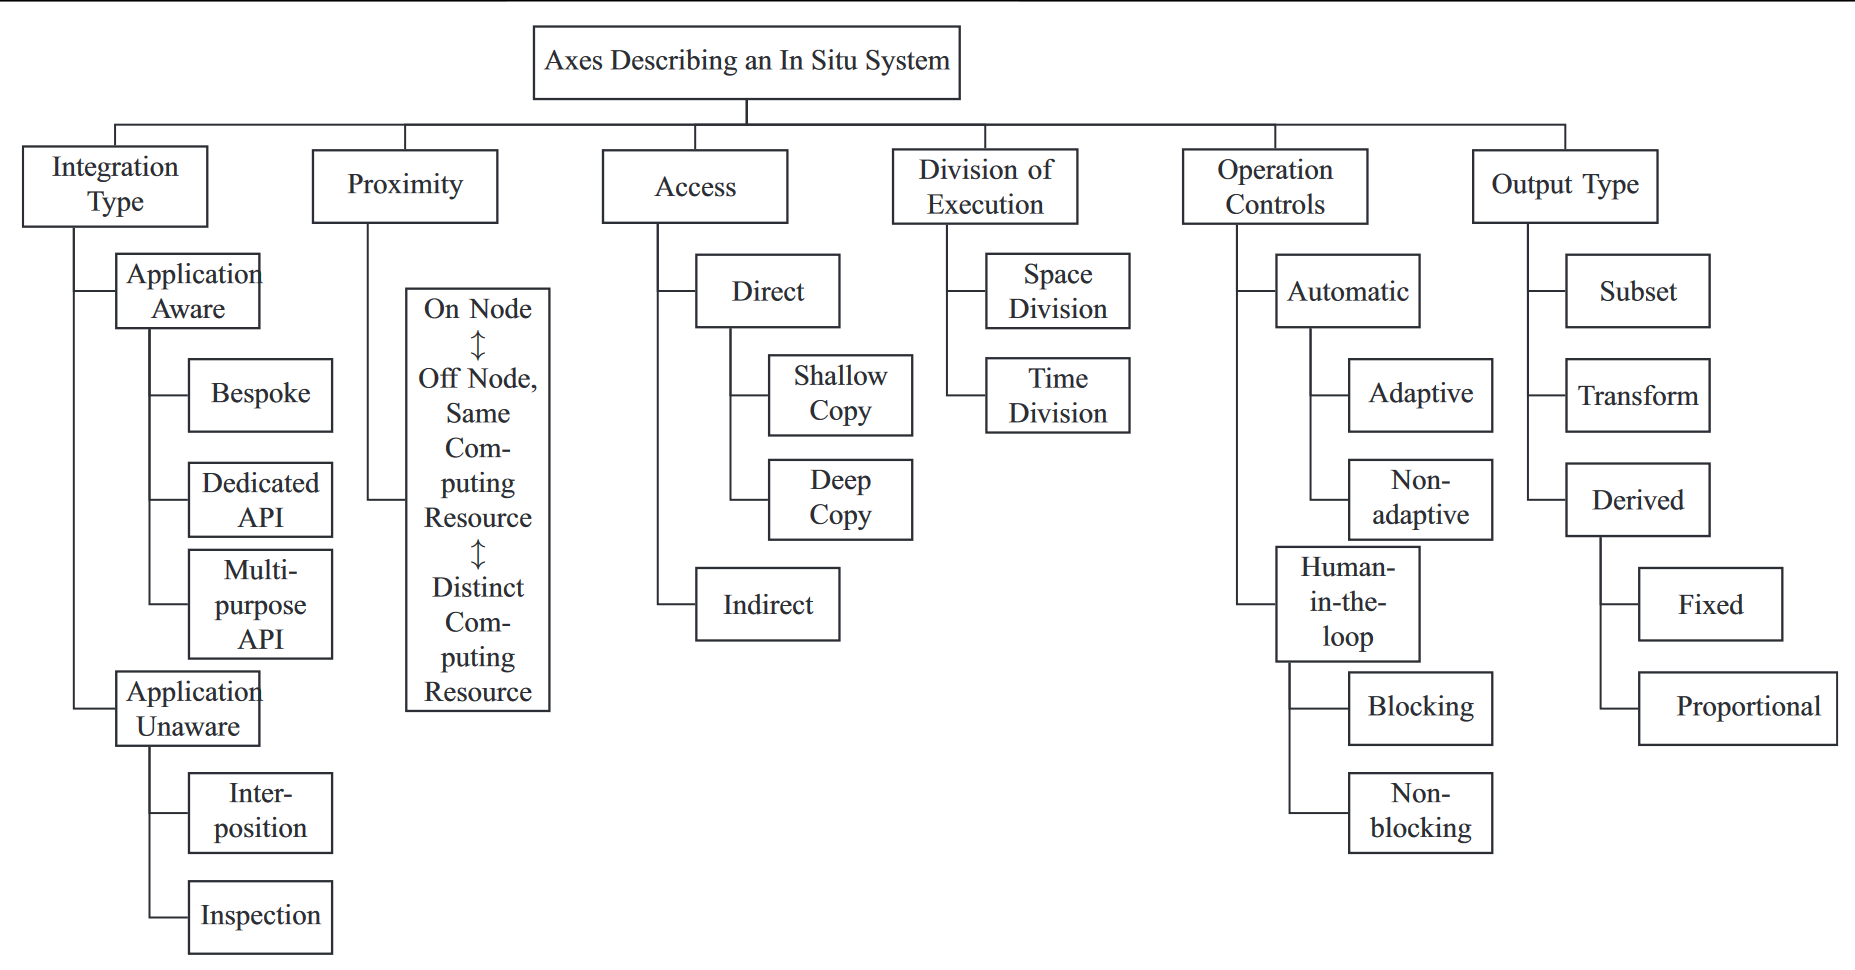
\includegraphics[width=\textwidth]{insitusystems}
  \label{fig:insitusystems}
  \caption{Características utilizadas para clasificar las bibliotecas in-situ. Imagen tomada de \cite{childs_terminology_2020} \colorbox{yellow}{TODO: Hacer mi propia versión}}
\end{figure}
\subsection{Caracterización de bibliotecas de análisis in-situ}
En la figura \ref{fig:insitusystems} se pueden observar los seis ejes con los que es posible realizar una caracterización las bibliotecas de visualización y análisis in-situ \cite{childs_terminology_2020}.
\begin{enumerate}
  \item Tipo de integración con la simulación.
  \item Proximidad del código de análisis y visualización de la simulación.
  \item El acceso de las bibliotecas a los punteros de los datos.
  \item La forma en la que se divide el tiempo o espacio de Ejecución.
  \item Controles que se tienen sobre la simulación mientras se ejecuta.
  \item Tipo de salida.
\end{enumerate}
\colorbox{yellow}{TODO: Explicar cada eje}
\subsection{Bibliotecas de análisis y visualización in-situ}
\subsubsection{ADIOS2}
Esta biblioteca \cite{Godoy2020} le permite al usuario realizar transferencias de datos entre unidades de ejecución de forma transparente, ya sea que es entre dos nodos de una supercomputadora conectadas por alguna red de interconexión como Infiniband, entre computadoras regulares conectadas por internet e incluso entre computadoras regulares y supercomputadoras.
Tiene tres APIs diseñadas con distintos niveles de abstracción.
\begin{itemize}
  \item El API de alto nivel está pensado para flujos de trabajo de análisis de datos. Tiene bindings para C++, Python y Matlab.
  \item El API de bajo nivel está diseñado para ser integrado en simulaciones de HPC. Está basado en MPI para reducir los costos de comunicación de red.
  \item El API privado permite desarrollar ADIOS con prácticas modernas de ingeniería de software.
\end{itemize}
\subsubsection{Catalyst}
Es una herramienta desarrollada por Kitware como un acompañante al software Paraview. Permite instrumentar el código mediante la implementación de un estándar llamado Conduit \cite{Ayachit2021}.


\colorbox{yellow}{TODO: Hablar específicamente de conduit, ParaView y VisIT}

\colorbox{yellow}{TODO: Relacionar las bibliotecas con la caracterización}
